\chapter{Appendix}

\section{Intuitive Analysis of PACUBIC}
\label{sec:appendix:pacubic}

\begin{figure*}[h]
\centering

\includegraphics[width=0.8\linewidth]{sidekick-paper/figures/cwnd/cwnd_legend.pdf}\\
\begin{subfigure}{0.32\linewidth}
	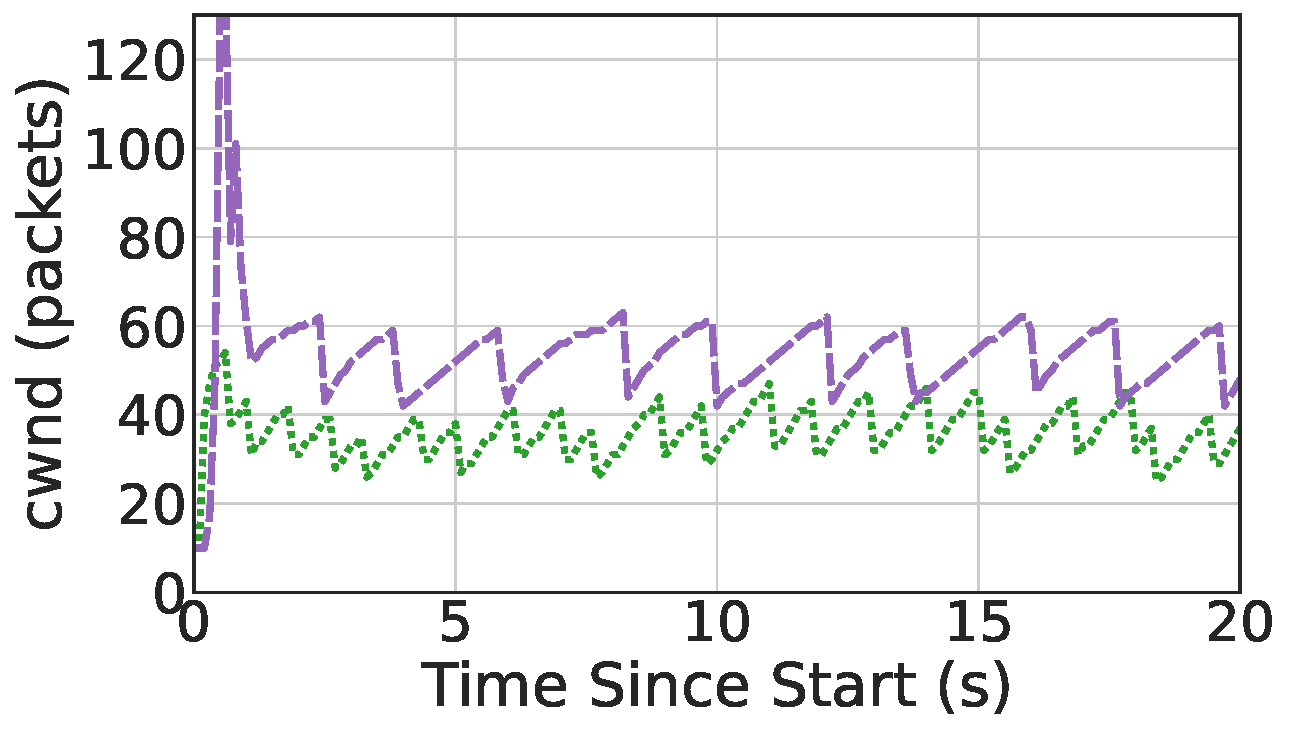
\includegraphics[width=\linewidth]{sidekick-paper/figures/cwnd/cwnd_split_loss0p.pdf}
	\caption{Split CUBIC, 0\% loss.}
	\label{fig:time-cwnd:split-loss0p}
\end{subfigure}
\begin{subfigure}{0.32\linewidth}
	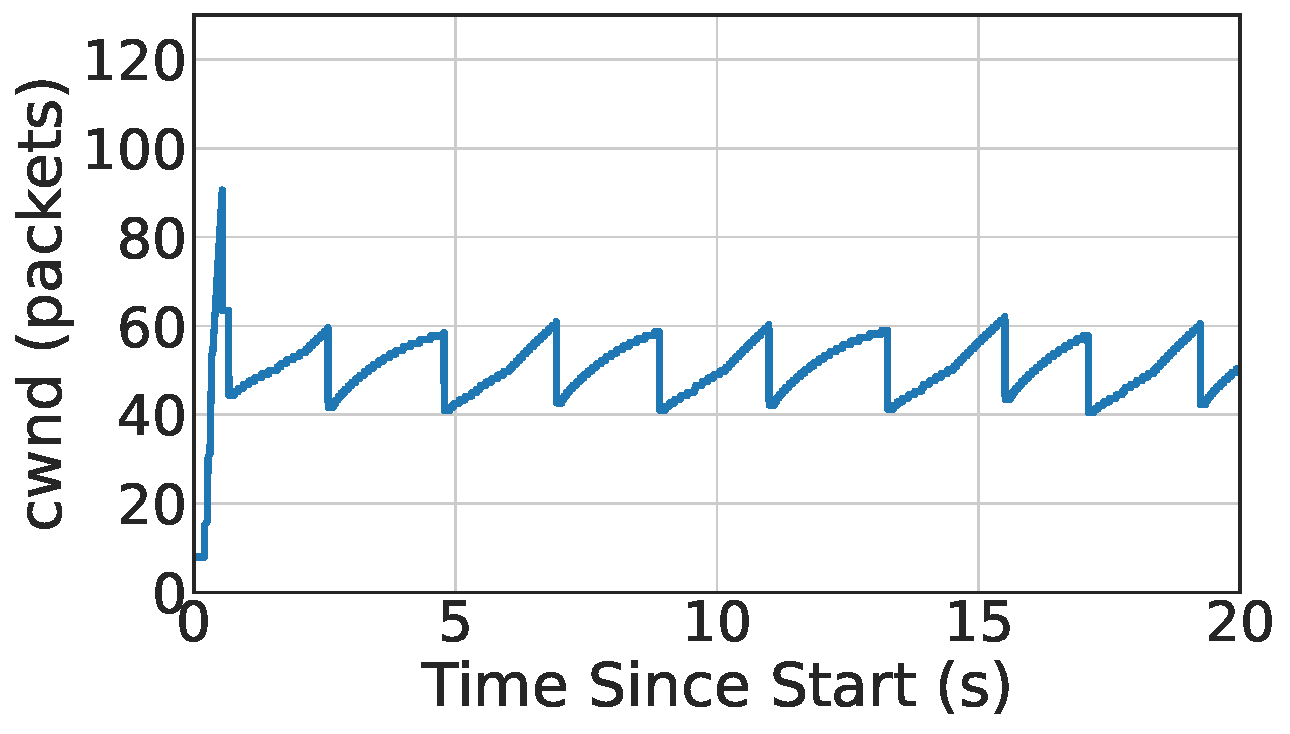
\includegraphics[width=\linewidth]{sidekick-paper/figures/cwnd/cwnd_pacubic_loss0p.pdf}
	\caption{PACUBIC, 0\% loss.}
	\label{fig:time-cwnd:pacubic-loss0p}
\end{subfigure}
\begin{subfigure}{0.32\linewidth}
	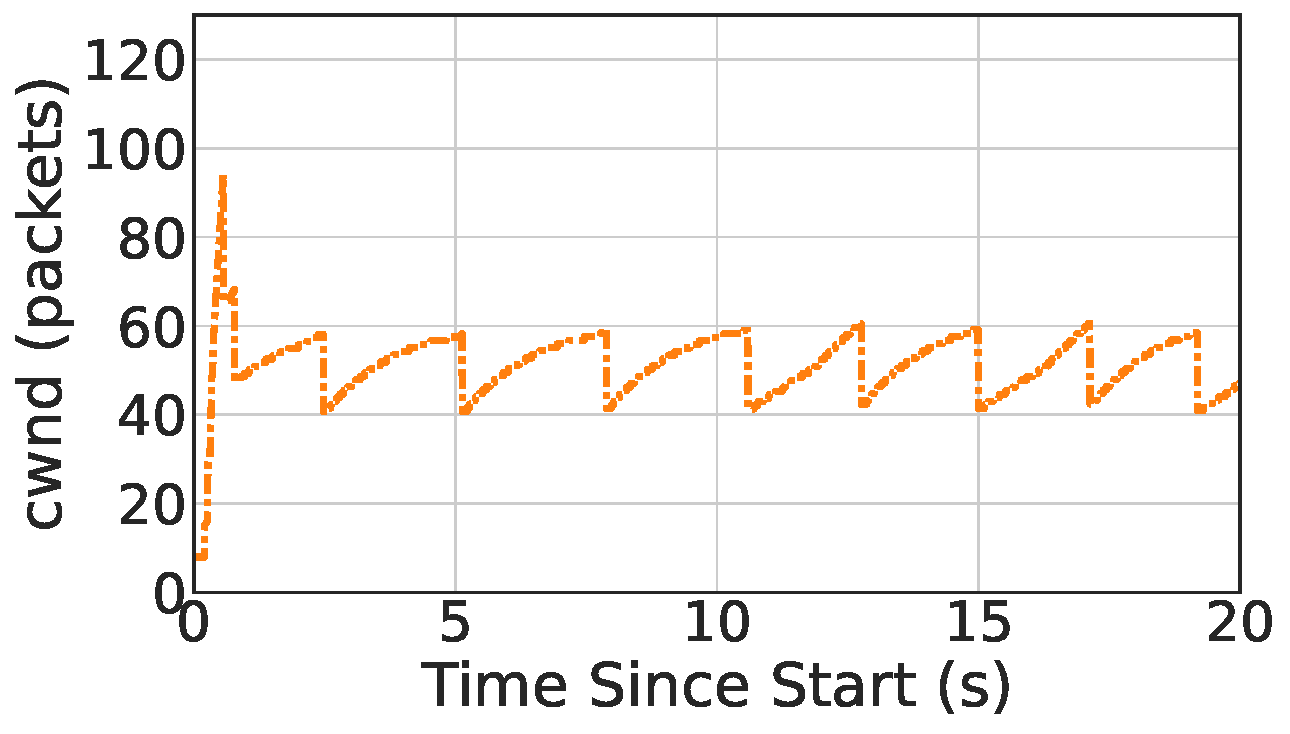
\includegraphics[width=\linewidth]{sidekick-paper/figures/cwnd/cwnd_cubic_loss0p.pdf}
	\caption{CUBIC, 0\% loss.}
	\label{fig:time-cwnd:cubic-loss0p}
\end{subfigure}
\begin{subfigure}{0.32\linewidth}
	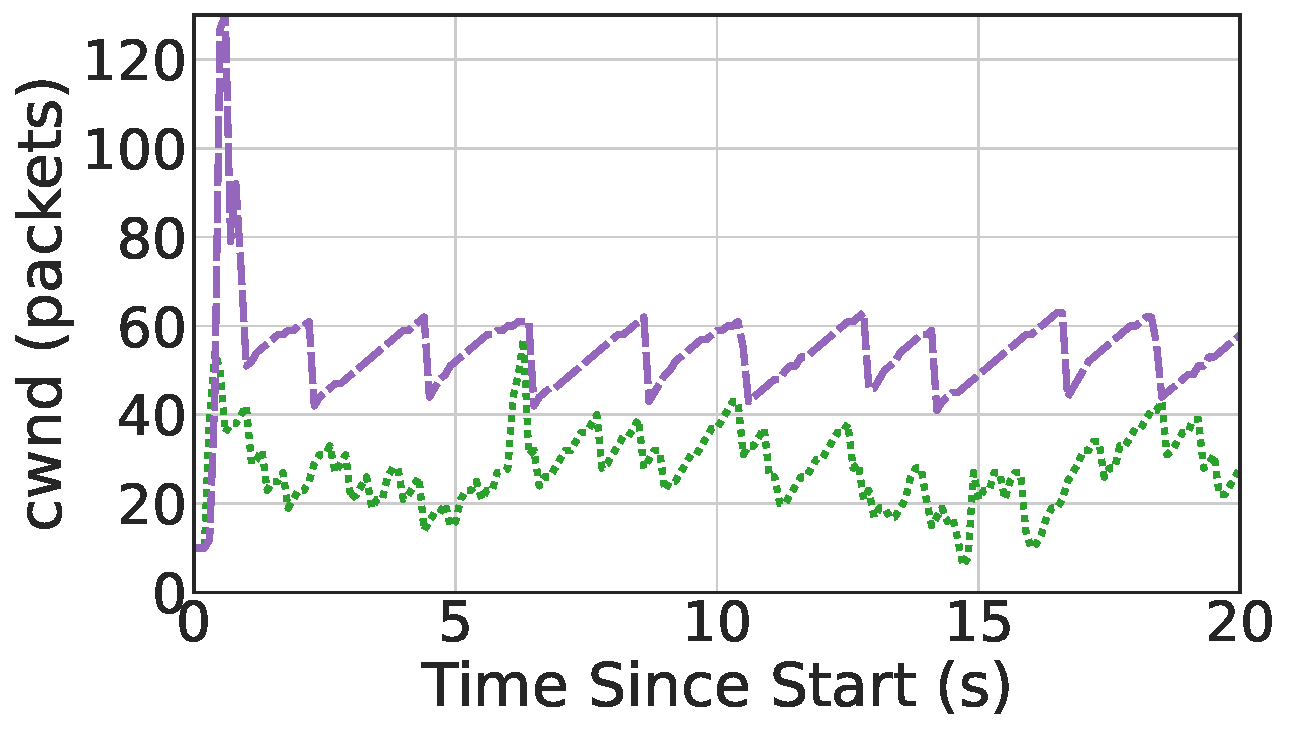
\includegraphics[width=\linewidth]{sidekick-paper/figures/cwnd/cwnd_split_loss1p.pdf}
	\caption{Split CUBIC, 1\% loss.}
	\label{fig:time-cwnd:split-loss1p}
\end{subfigure}
\begin{subfigure}{0.32\linewidth}
	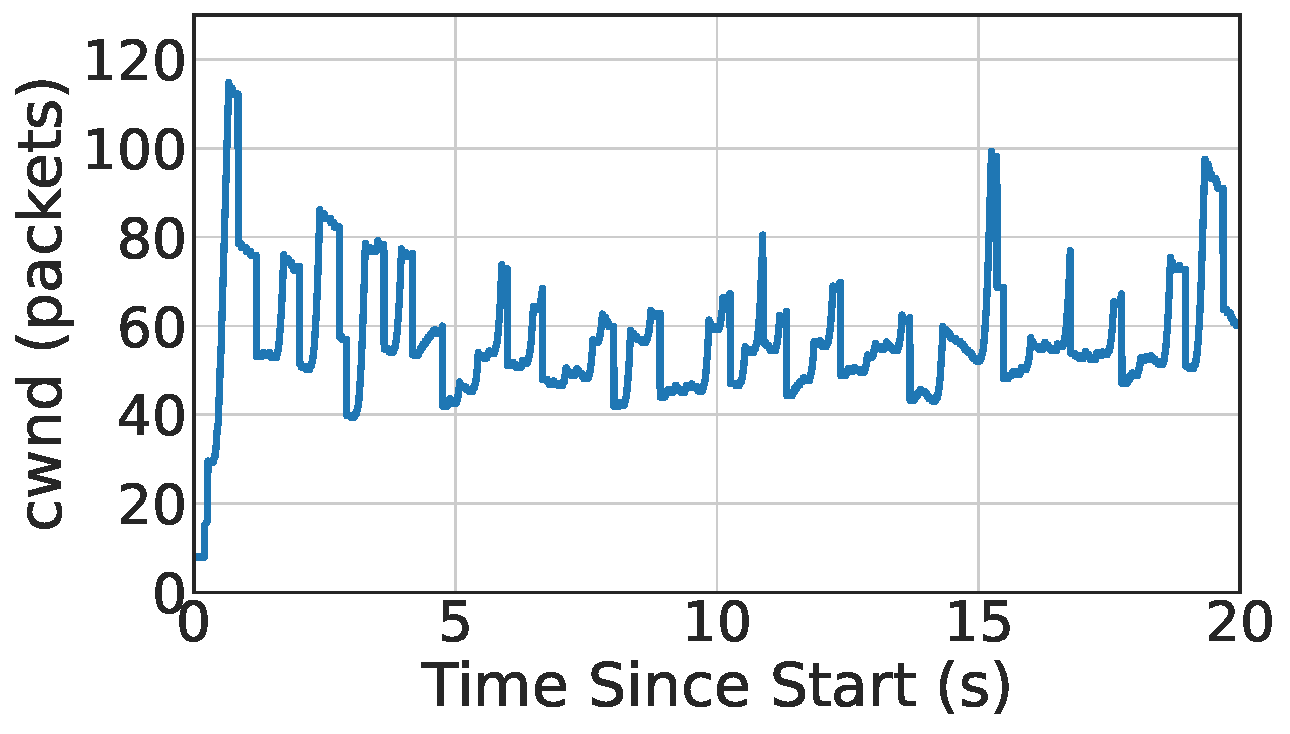
\includegraphics[width=\linewidth]{sidekick-paper/figures/cwnd/cwnd_pacubic_loss1p.pdf}
	\caption{PACUBIC, 1\% loss.}
	\label{fig:time-cwnd:pacubic-loss1p}
\end{subfigure}
\begin{subfigure}{0.32\linewidth}
	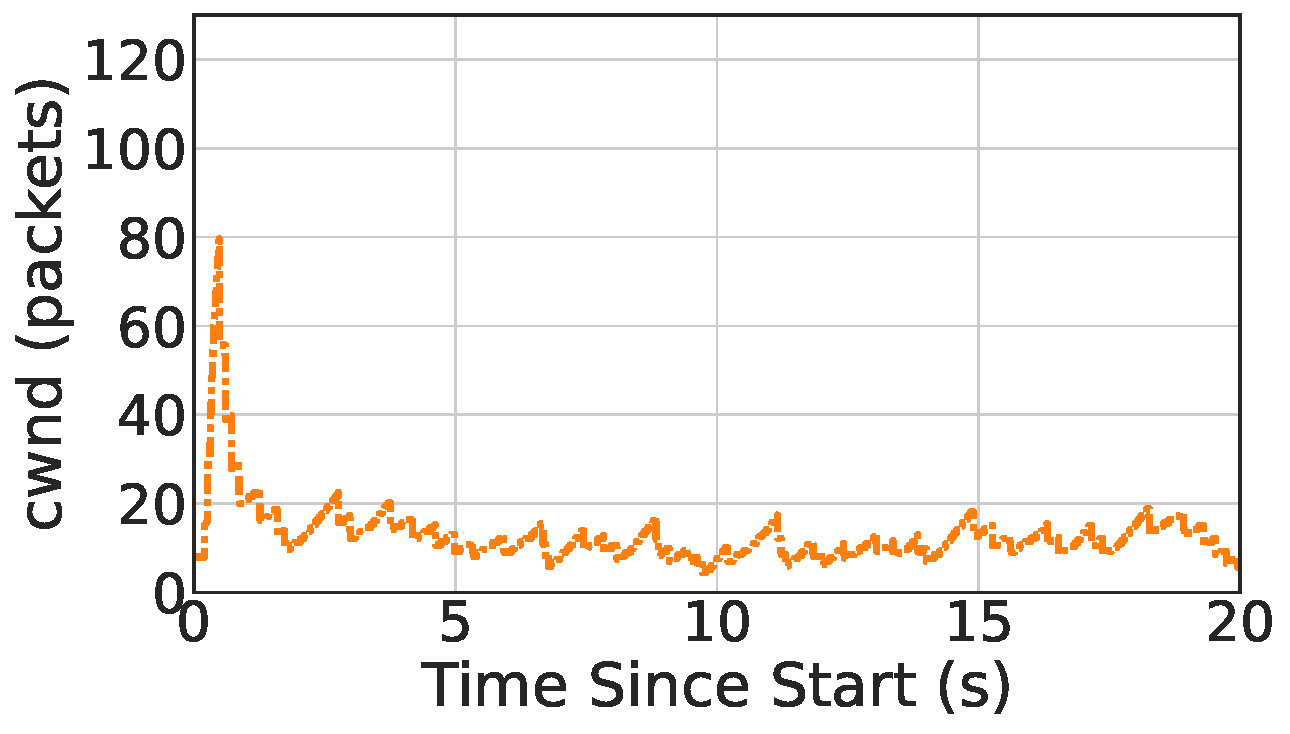
\includegraphics[width=\linewidth]{sidekick-paper/figures/cwnd/cwnd_cubic_loss1p.pdf}
	\caption{CUBIC, 1\% loss.}
	\label{fig:time-cwnd:cubic-loss1p}
\end{subfigure}
\caption{Congestion window of a long-running upload in Scenario \#2
(\Cref{tab:experimental-scenarios}) with $0\%$ and $1\%$ loss on the near
path segmenet.
The cwnd is measured at the data sender,
except for split CUBIC whose split connection also has a cwnd at the proxy.
PACUBIC reacts to every congestion event while keeping the cwnd high.
CUBIC performs poorly when there is loss on the near path segment.
CUBIC and PACUBIC are implemented in QUIC, while split CUBIC is implemented
in TCP using a PEP.
}
\label{fig:time-cwnd}
\end{figure*}

Here, we dive deeper into the intuition behind the PACUBIC constants
(\Cref{sec:sidekick:protocol:sender-behavior}), including how they were derived and why the PACUBIC
algorithm achieves similar congestion behavior to the CUBIC algorithm in a split
connection---we call this behavior ``split CUBIC''.

Consider the same network topology as \Cref{fig:sc-protocols} in which a
data sender uploads a large file to a data receiver, with help from a Sidekick
proxy in the middle of the connection. The near path segment connects the sender
to the proxy, and the far path segment connects the proxy to the receiver.
The near segment is low-delay with varying random loss, and the far segment is
high-delay with no random loss. The far segment is the bottleneck link in terms
of bandwidth.
The actual link parameters are the same as in Scenario \#2 of
\Cref{tab:experimental-scenarios}.

We first discuss how split CUBIC would behave in this setting to conceptually
motivate PACUBIC.
Consider the congestion windows of each half of the
split connection, one taken at the data sender and one at the proxy
(\Cref{fig:time-cwnd:split-loss0p,fig:time-cwnd:split-loss1p}).
The far path segment experiences only congestive loss,
leading the window at the proxy to fluctuate around the segment's BDP
regardless of the loss on the near path segment.
The window at the data sender independently determines whether the packets
that reach the proxy will be able to fully utilize the window set at the far
path segment. The data sender is able to achieve this at low random loss rates, but
becomes the bottleneck as loss rates increase (\Cref{fig:loss-vs-tput}).

While split CUBIC has two windows, PACUBIC only has one
window representing the in-flight bytes of the end-to-end connection.
PACUBIC considers loss detected from both quACKs and end-to-end ACKs.
Conceptually, we want an algorithm that would enable PACUBIC's single
congestion window to match the sum of CUBIC's two congestion windows, or
the total number of in-flight bytes.
% That is the motivation behind adjusting the window proportionally to the
% number of in-flight bytes on each path segment, depending on where the loss occurred.

With no random loss on the near path segment, PACUBIC (\Cref{fig:time-cwnd:pacubic-loss0p})
behaves the same as normal CUBIC (\Cref{fig:time-cwnd:cubic-loss0p}).
The congestion window is entirely governed by end-to-end ACKs since
the far path segment is the bottleneck link. Note that while the sender may be
able to deduce that a loss occurred on the far path segment by combining info from
the quACK with the end-to-end ACK, PACUBIC conservatively treats the loss as
occurring anywhere on the path.

With some random loss on the near path segment, PACUBIC grows and reduces cwnd
based on where the last congestion event occurs (\Cref{fig:time-cwnd:pacubic-loss1p}).
Note that if the congestion window $cwnd$
represents the bytes in-flight in the end-to-end connection, then
$r \cdot cwnd$ represents the proportion of bytes in-flight on the near
path segment. At a high level, if the data sender discovers loss
on the near path segment via the quACK, it holds the $(1-r)\cdot cwnd$ portion of
the ``far window'' constant while applying the CUBIC algorithm to the remaining
$r \cdot w_{max}$ of the ``near window,'' representing the bottleneck link.

Mathematically, instead of reducing $w_{max}$, the window size just before the
last reduction, by $(1-\beta^*) \cdot w_{max}$, PACUBIC reduces it by only
$[1 - (1-r(1-\beta^*))] \cdot w_{max} = r(1-\beta^*) \cdot w_{max}$.
That is $r$ times the original reduction, a \emph{smaller} amount.
We use the RTT ratio $r$ (near path segment to end-to-end)
% indicating the RTT ratio of near path segment vs.~far path segment)
as a proxy for the ratio of the number of in-flight bytes.

Similarly, instead of using a cubic growth function with scaling factor $C^*$
and inflection point $K = K^* = \sqrt[3]{w_{max}(1-\beta^*)/C^*}$,
we use a larger scaling factor $C = C^*/r^3$
and thus a shorter inflection point
\[
K = \sqrt[3]{\frac{w_{max}(1-\beta)}{C}}
= \sqrt[3]{\frac{r\cdot w_{max}(1-\beta^*)}{C^* / r^3}}
= r^{4/3} \cdot K^*.
\]
The shorter inflection point leads the congestion window to \emph{grow more
quickly} since the sender also reacts to feedback about loss more quickly over
the low-delay link.
% Since
% similarly proportional to $w_{max}$, so with $C'$, we both reduce the inflection
% point $K$ and the growth rate $C$ of the function proportionally to the
% number of bytes in-flight on the near path segment.

At times, there can be loss detected both in quACKs and in end-to-end ACKs.
The end-to-end ACKs have a greater effect since they reduce the congestion
window by a larger proportion, until the remaining path segment with loss is the
bottleneck link. In this scenario with loss, the bottleneck link at equilibrium
is the near path segment.
At this point, the quACK primarily determines the congestion window updates.
If the far path segment were to become the bottleneck again, the data sender would
detect a congestion event via the end-to-end ACK.

PACUBIC has several limitations. Although it beats end-to-end CUBIC, it
still performs worse than split CUBIC, especially at
high loss rates (\Cref{fig:loss-vs-tput}). Also, it doesn't consider loss on the
far path segment any differently than original CUBIC, unlike split CUBIC
which treats the two split connections independently. PACUBIC
emulates the congestion control behavior and fairness of split CUBIC
fairly well as a heuristic, but would benefit from an analysis in a
wider variety of network scenarios. It would also benefit from a side-by-side
fairness comparison against other congestion control algorithms that perform
well in the same scenarios. We'd like the primary takeaway of PACUBIC to be
that knowing where loss occurs can cleverly inform congestion control.

\section{Congestion Control Scheme Characterizations}
\label{sec:appendix:heatmaps}

We present the raw data for our characterizations of each
congestion control scheme.

\begin{figure*}[ht]
    \centering
    \begin{subfigure}[b]{0.22\linewidth}
        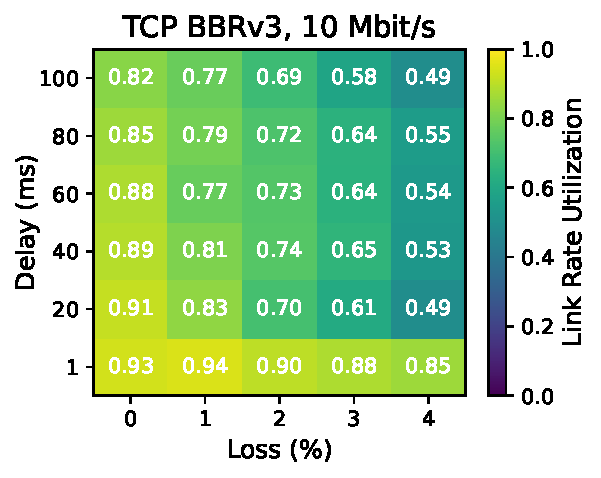
\includegraphics[width=\linewidth,trim={0 0 2cm 0},clip]{splitting-paper/figures/heatmaps/heatmap_tcp_bbr3_10mbps.pdf}
        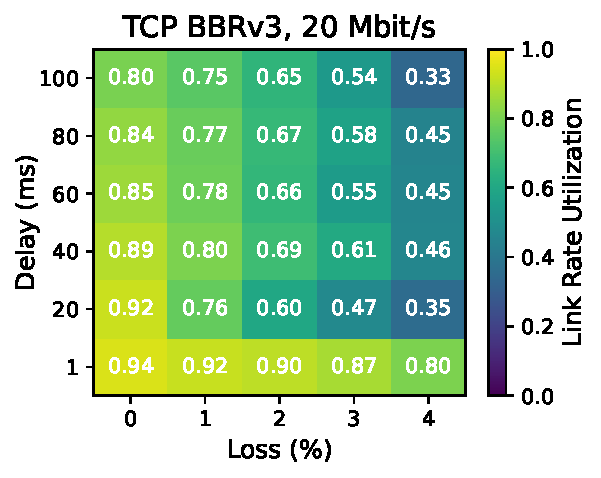
\includegraphics[width=\linewidth,trim={0 0 2cm 0},clip]{splitting-paper/figures/heatmaps/heatmap_tcp_bbr3_20mbps.pdf}
        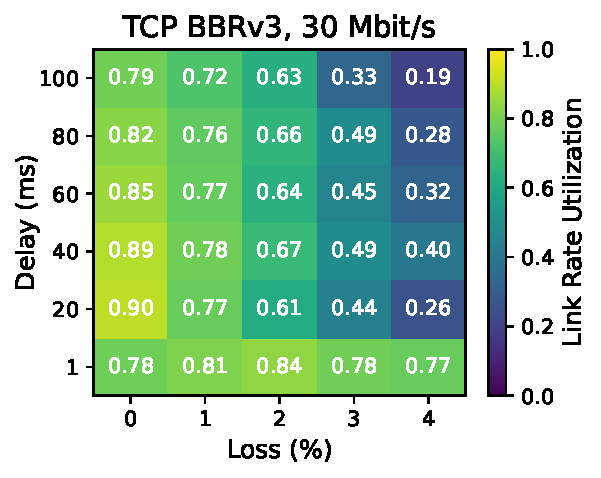
\includegraphics[width=\linewidth,trim={0 0 2cm 0},clip]{splitting-paper/figures/heatmaps/heatmap_tcp_bbr3_30mbps.pdf}
        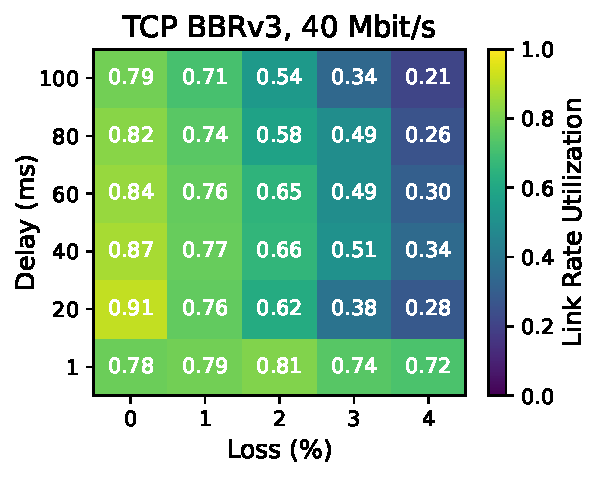
\includegraphics[width=\linewidth,trim={0 0 2cm 0},clip]{splitting-paper/figures/heatmaps/heatmap_tcp_bbr3_40mbps.pdf}
        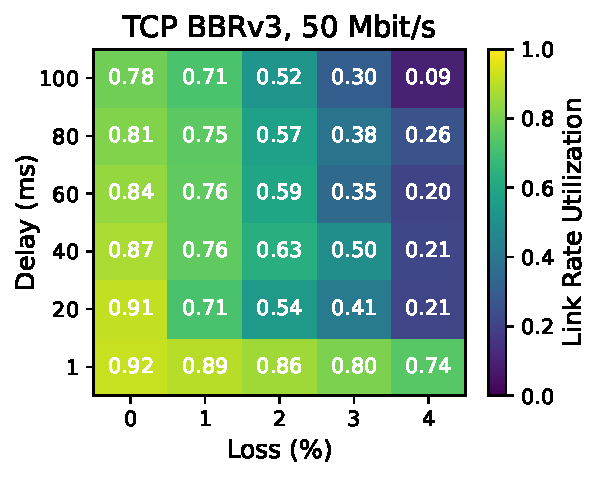
\includegraphics[width=\linewidth,trim={0 0 2cm 0},clip]{splitting-paper/figures/heatmaps/heatmap_tcp_bbr3_50mbps.pdf}
        \caption{Linux TCP.}
    \end{subfigure}
    \begin{subfigure}[b]{0.22\linewidth}
        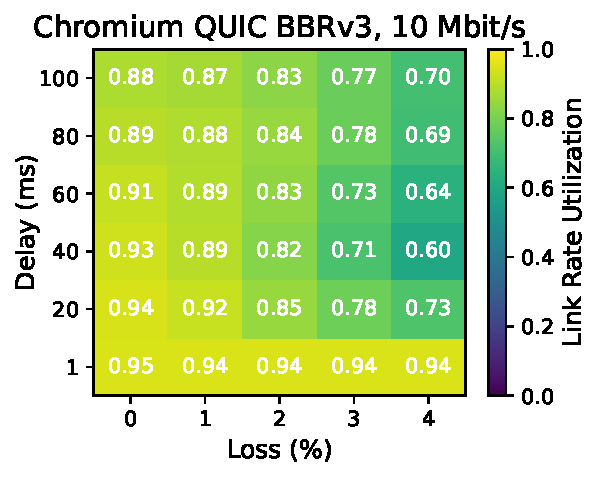
\includegraphics[width=\linewidth,trim={0 0 2cm 0},clip]{splitting-paper/figures/heatmaps/heatmap_quic_bbr3_10mbps.pdf}
        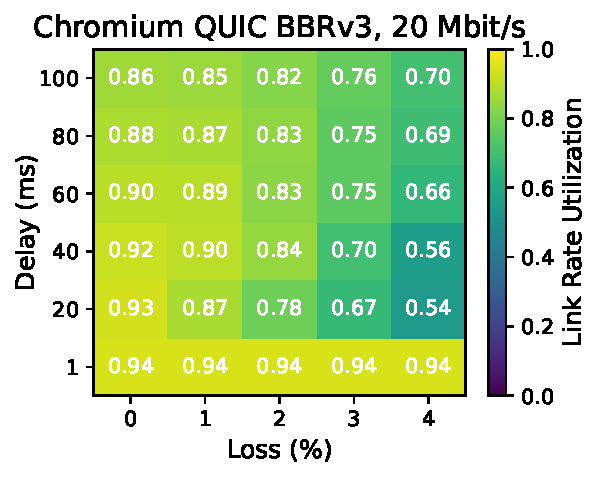
\includegraphics[width=\linewidth,trim={0 0 2cm 0},clip]{splitting-paper/figures/heatmaps/heatmap_quic_bbr3_20mbps.pdf}
        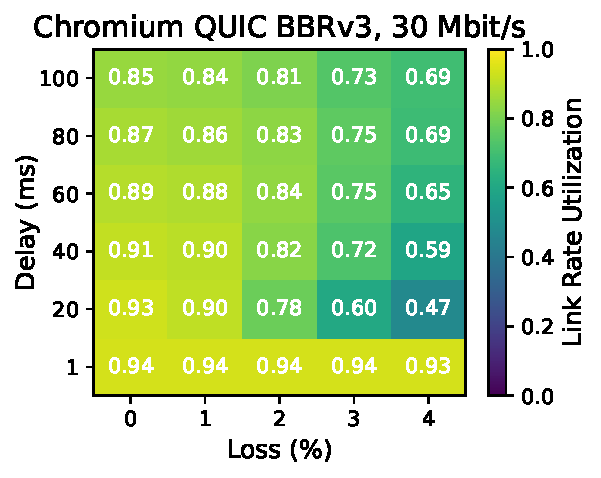
\includegraphics[width=\linewidth,trim={0 0 2cm 0},clip]{splitting-paper/figures/heatmaps/heatmap_quic_bbr3_30mbps.pdf}
        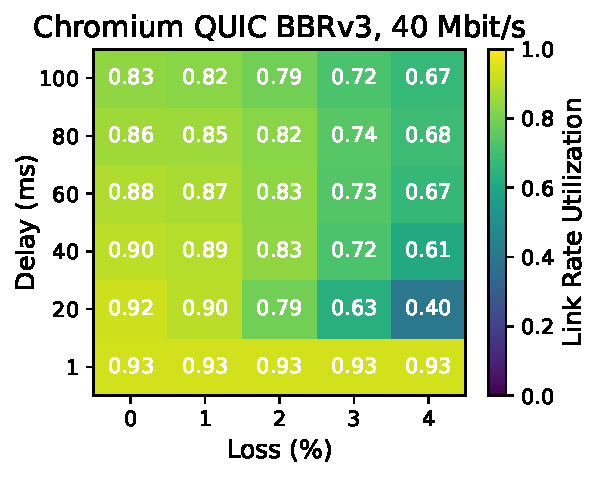
\includegraphics[width=\linewidth,trim={0 0 2cm 0},clip]{splitting-paper/figures/heatmaps/heatmap_quic_bbr3_40mbps.pdf}
        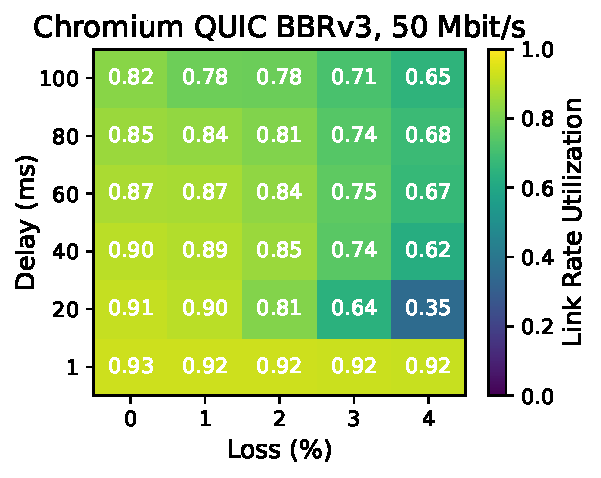
\includegraphics[width=\linewidth,trim={0 0 2cm 0},clip]{splitting-paper/figures/heatmaps/heatmap_quic_bbr3_50mbps.pdf}
        \caption{Google \texttt{quiche}.}
    \end{subfigure}
    \begin{subfigure}[b]{0.22\linewidth}
        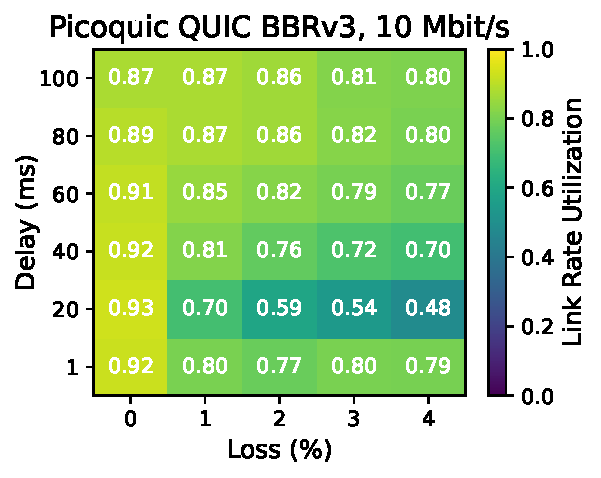
\includegraphics[width=\linewidth,trim={0 0 2cm 0},clip]{splitting-paper/figures/heatmaps/heatmap_picoquic_bbr3_10mbps.pdf}
        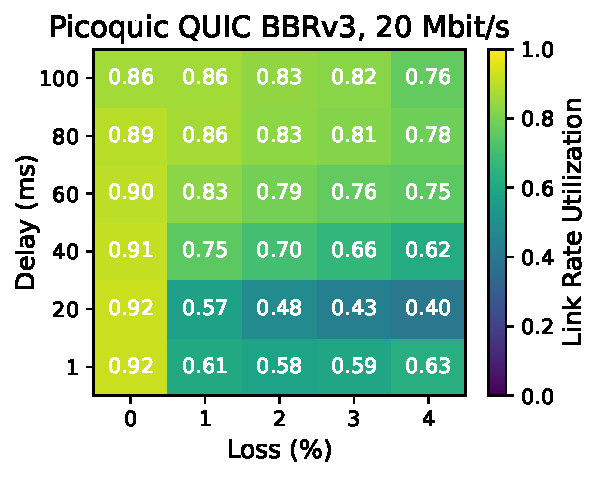
\includegraphics[width=\linewidth,trim={0 0 2cm 0},clip]{splitting-paper/figures/heatmaps/heatmap_picoquic_bbr3_20mbps.pdf}
        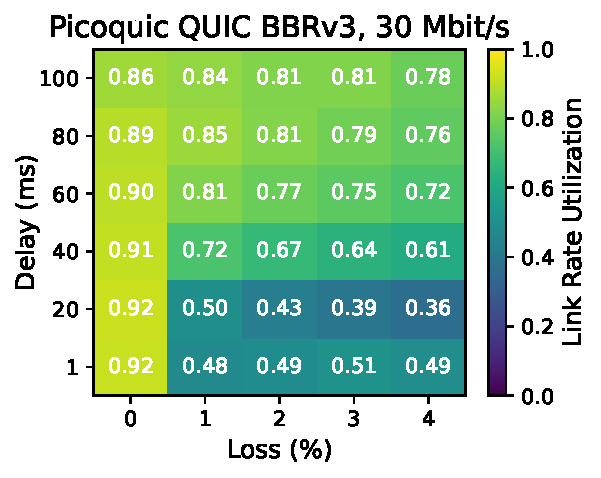
\includegraphics[width=\linewidth,trim={0 0 2cm 0},clip]{splitting-paper/figures/heatmaps/heatmap_picoquic_bbr3_30mbps.pdf}
        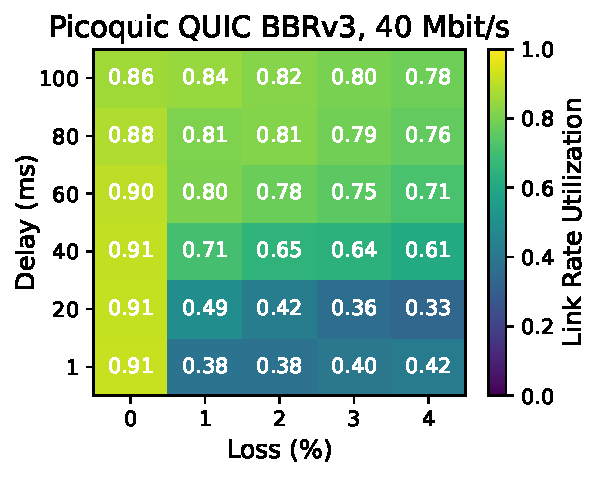
\includegraphics[width=\linewidth,trim={0 0 2cm 0},clip]{splitting-paper/figures/heatmaps/heatmap_picoquic_bbr3_40mbps.pdf}
        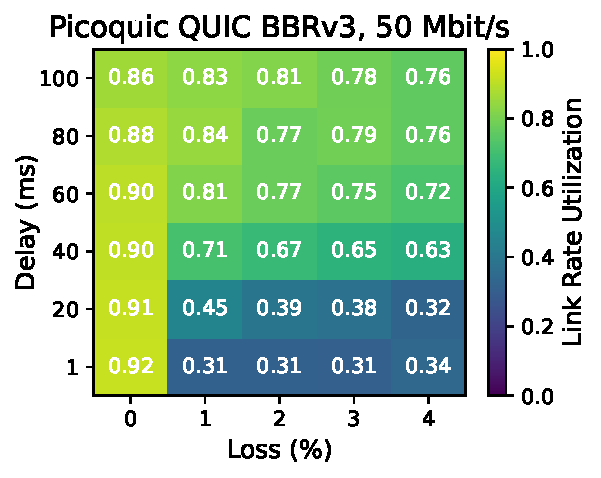
\includegraphics[width=\linewidth,trim={0 0 2cm 0},clip]{splitting-paper/figures/heatmaps/heatmap_picoquic_bbr3_50mbps.pdf}
        \caption{\texttt{picoquic}.}
    \end{subfigure}
    \begin{subfigure}[b]{0.89cm}
        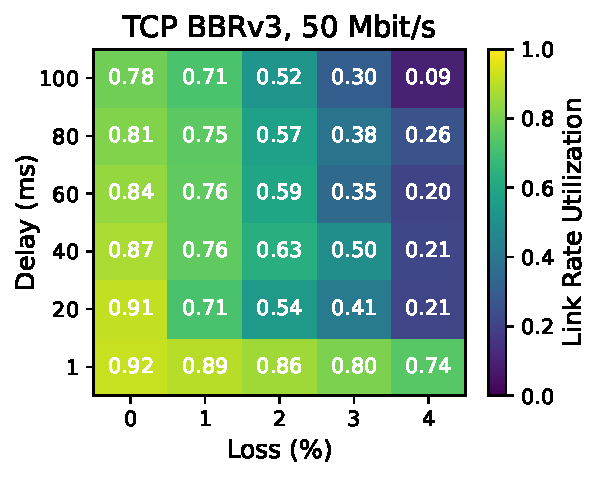
\includegraphics[width=\linewidth,trim={8cm 0 0 0},clip]{splitting-paper/figures/heatmaps/heatmap_tcp_bbr3_50mbps.pdf}
        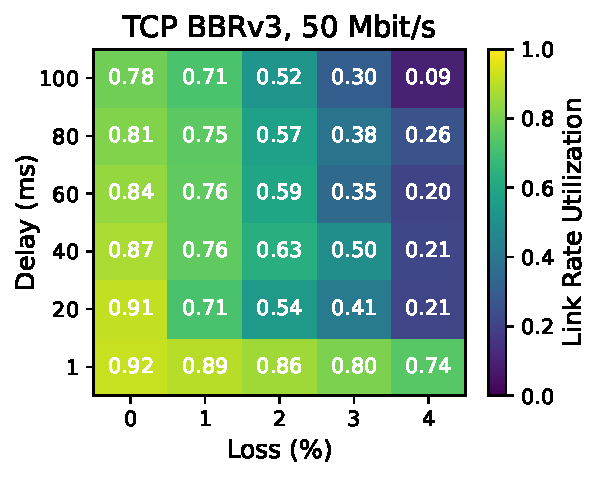
\includegraphics[width=\linewidth,trim={8cm 0 0 0},clip]{splitting-paper/figures/heatmaps/heatmap_tcp_bbr3_50mbps.pdf}
        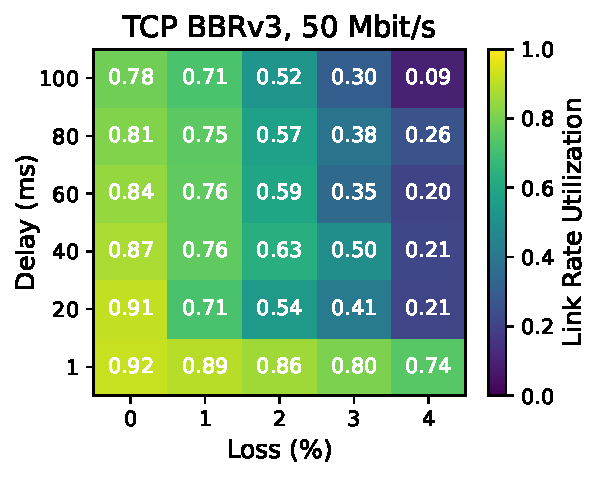
\includegraphics[width=\linewidth,trim={8cm 0 0 0},clip]{splitting-paper/figures/heatmaps/heatmap_tcp_bbr3_50mbps.pdf}
        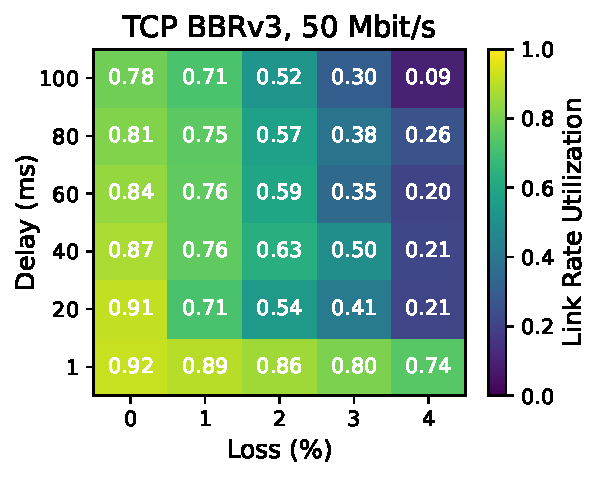
\includegraphics[width=\linewidth,trim={8cm 0 0 0},clip]{splitting-paper/figures/heatmaps/heatmap_tcp_bbr3_50mbps.pdf}
        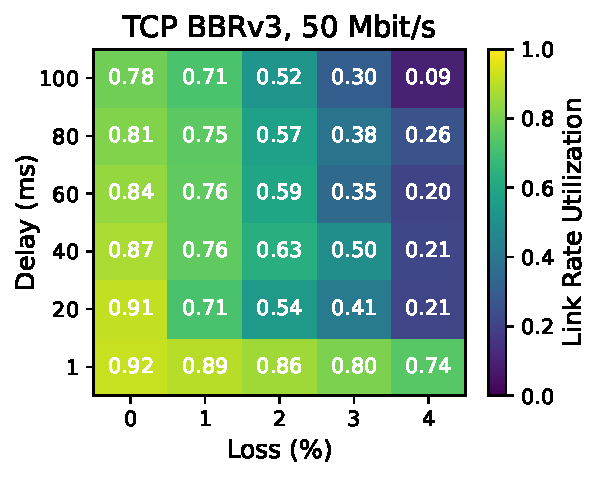
\includegraphics[width=\linewidth,trim={8cm 0 0 0},clip]{splitting-paper/figures/heatmaps/heatmap_tcp_bbr3_50mbps.pdf}
        \vspace*{0.2cm}
    \end{subfigure}
    \caption{BBRv3.}
\end{figure*}

\begin{figure*}[ht]
    \centering
    \begin{subfigure}[b]{0.22\linewidth}
        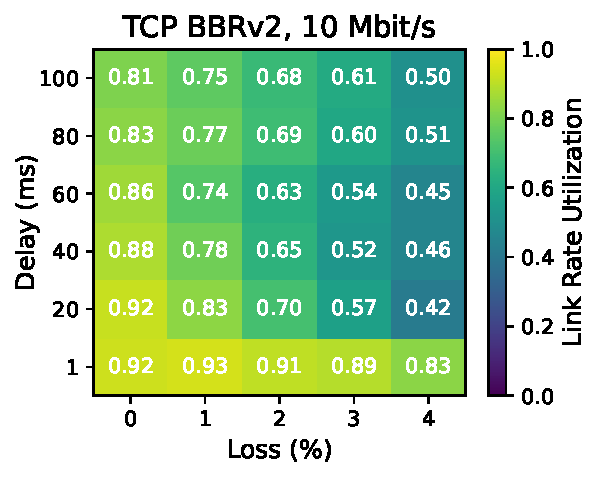
\includegraphics[width=\linewidth,trim={0 0 2cm 0},clip]{splitting-paper/figures/heatmaps/heatmap_tcp_bbr2_10mbps.pdf}
        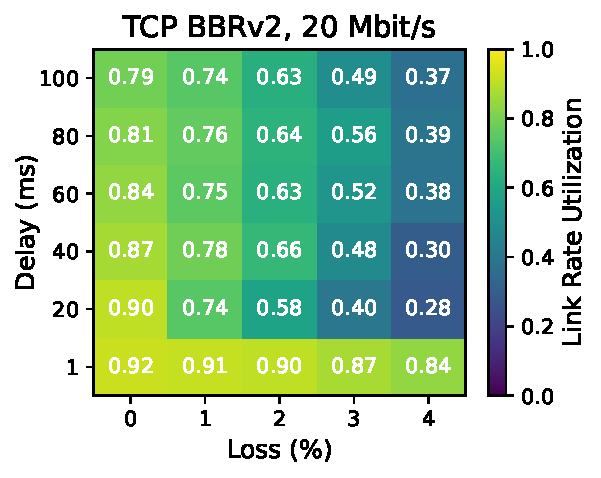
\includegraphics[width=\linewidth,trim={0 0 2cm 0},clip]{splitting-paper/figures/heatmaps/heatmap_tcp_bbr2_20mbps.pdf}
        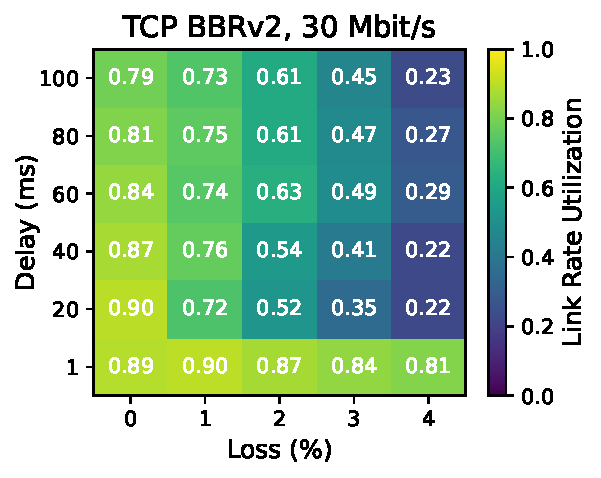
\includegraphics[width=\linewidth,trim={0 0 2cm 0},clip]{splitting-paper/figures/heatmaps/heatmap_tcp_bbr2_30mbps.pdf}
        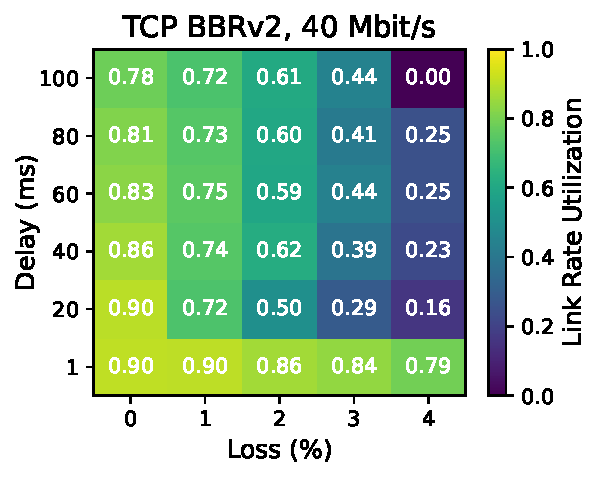
\includegraphics[width=\linewidth,trim={0 0 2cm 0},clip]{splitting-paper/figures/heatmaps/heatmap_tcp_bbr2_40mbps.pdf}
        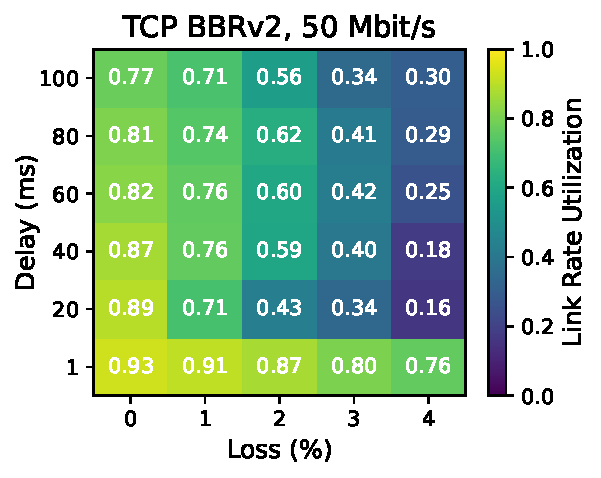
\includegraphics[width=\linewidth,trim={0 0 2cm 0},clip]{splitting-paper/figures/heatmaps/heatmap_tcp_bbr2_50mbps.pdf}
        \caption{Linux TCP.}
    \end{subfigure}
    \begin{subfigure}[b]{0.22\linewidth}
        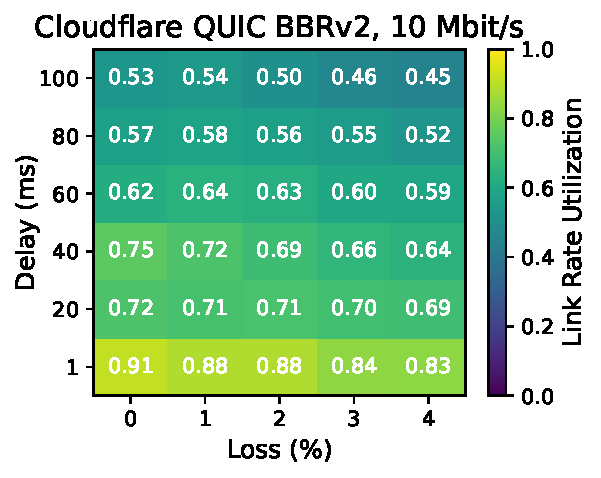
\includegraphics[width=\linewidth,trim={0 0 2cm 0},clip]{splitting-paper/figures/heatmaps/heatmap_quiche_bbr2_10mbps.pdf}
        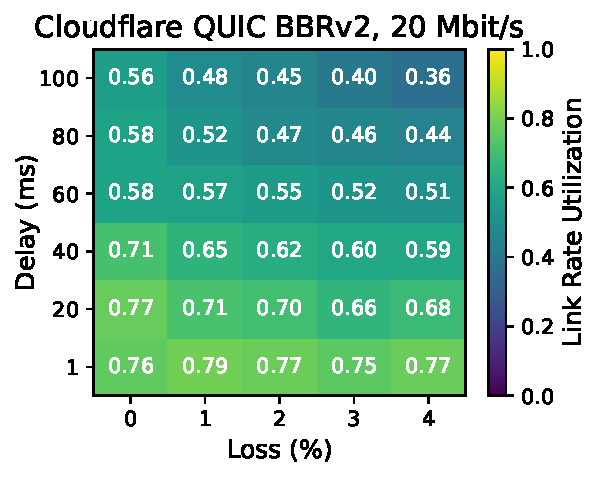
\includegraphics[width=\linewidth,trim={0 0 2cm 0},clip]{splitting-paper/figures/heatmaps/heatmap_quiche_bbr2_20mbps.pdf}
        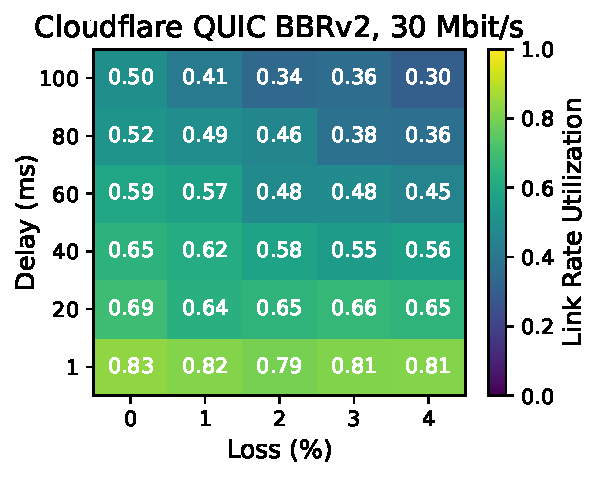
\includegraphics[width=\linewidth,trim={0 0 2cm 0},clip]{splitting-paper/figures/heatmaps/heatmap_quiche_bbr2_30mbps.pdf}
        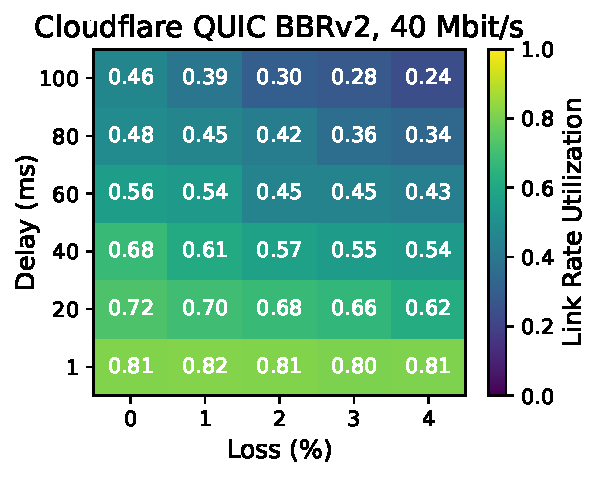
\includegraphics[width=\linewidth,trim={0 0 2cm 0},clip]{splitting-paper/figures/heatmaps/heatmap_quiche_bbr2_40mbps.pdf}
        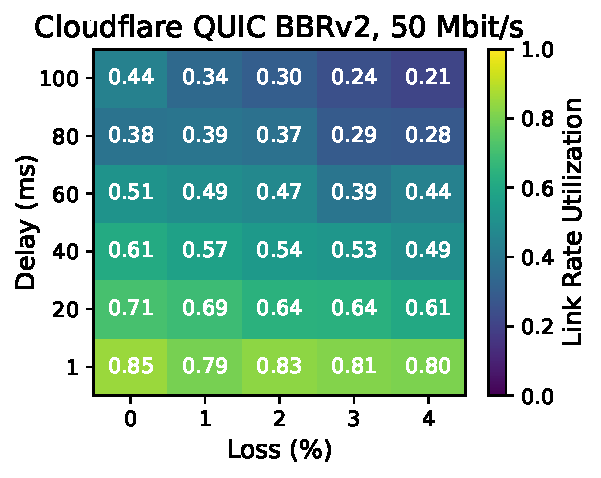
\includegraphics[width=\linewidth,trim={0 0 2cm 0},clip]{splitting-paper/figures/heatmaps/heatmap_quiche_bbr2_50mbps.pdf}
        \caption{Cloudflare \texttt{quiche}.}
    \end{subfigure}
    \begin{subfigure}[b]{0.89cm}
        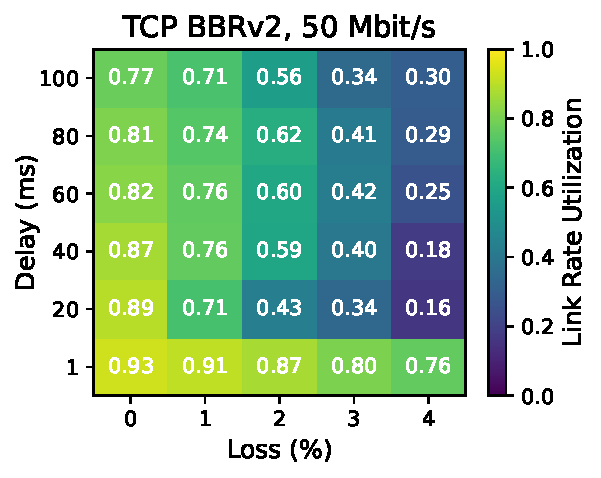
\includegraphics[width=\linewidth,trim={8cm 0 0 0},clip]{splitting-paper/figures/heatmaps/heatmap_tcp_bbr2_50mbps.pdf}
        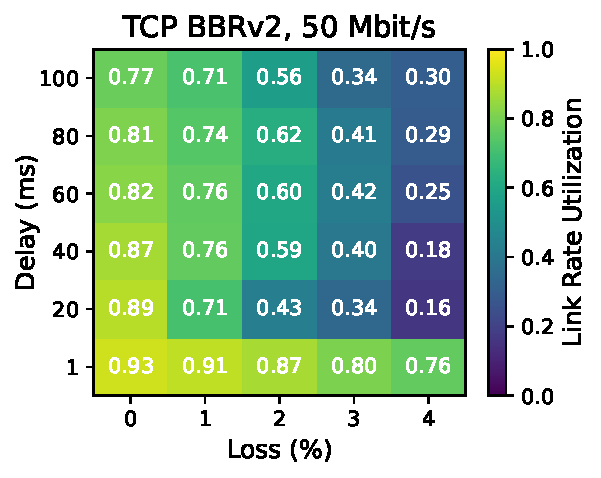
\includegraphics[width=\linewidth,trim={8cm 0 0 0},clip]{splitting-paper/figures/heatmaps/heatmap_tcp_bbr2_50mbps.pdf}
        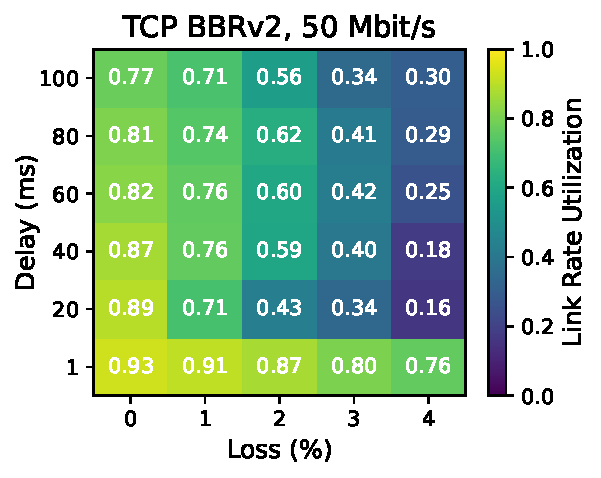
\includegraphics[width=\linewidth,trim={8cm 0 0 0},clip]{splitting-paper/figures/heatmaps/heatmap_tcp_bbr2_50mbps.pdf}
        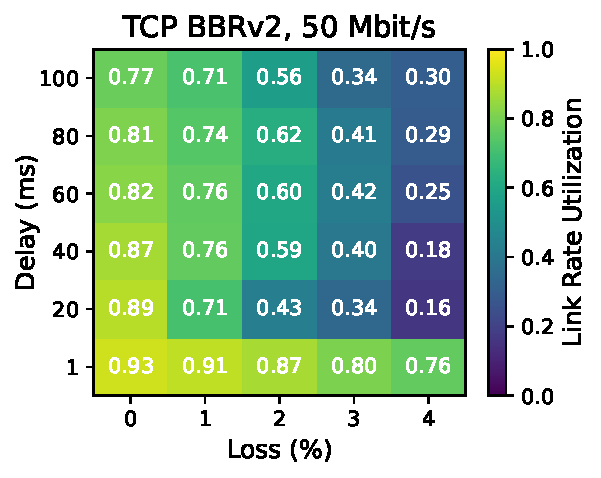
\includegraphics[width=\linewidth,trim={8cm 0 0 0},clip]{splitting-paper/figures/heatmaps/heatmap_tcp_bbr2_50mbps.pdf}
        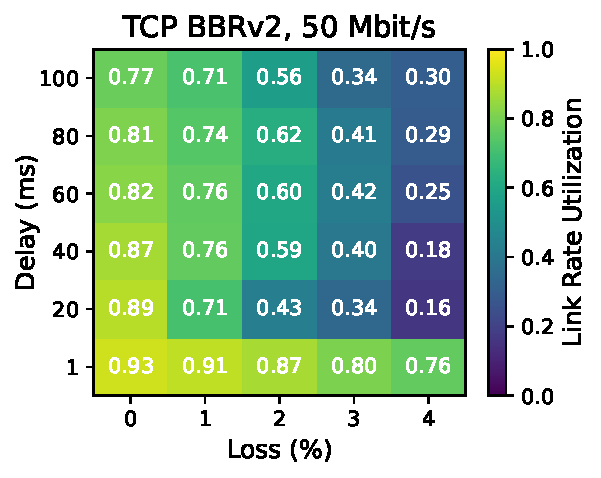
\includegraphics[width=\linewidth,trim={8cm 0 0 0},clip]{splitting-paper/figures/heatmaps/heatmap_tcp_bbr2_50mbps.pdf}
        \vspace*{0.2cm}
    \end{subfigure}
    \caption{BBRv2.}
\end{figure*}

\begin{figure*}[ht]
    \centering
    \begin{subfigure}[b]{0.22\linewidth}
        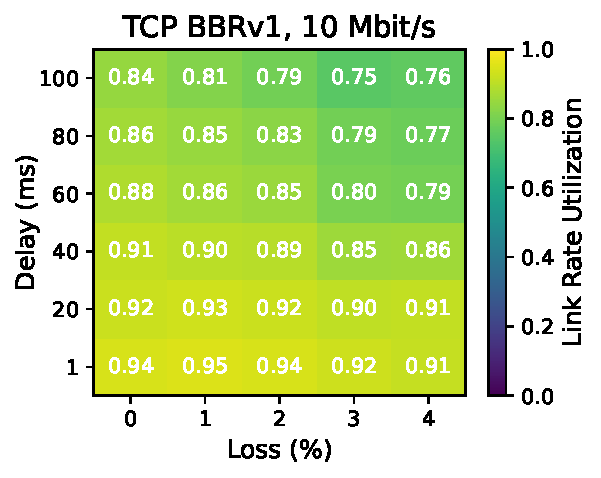
\includegraphics[width=\linewidth,trim={0 0 2cm 0},clip]{splitting-paper/figures/heatmaps/heatmap_tcp_bbr1_10mbps.pdf}
        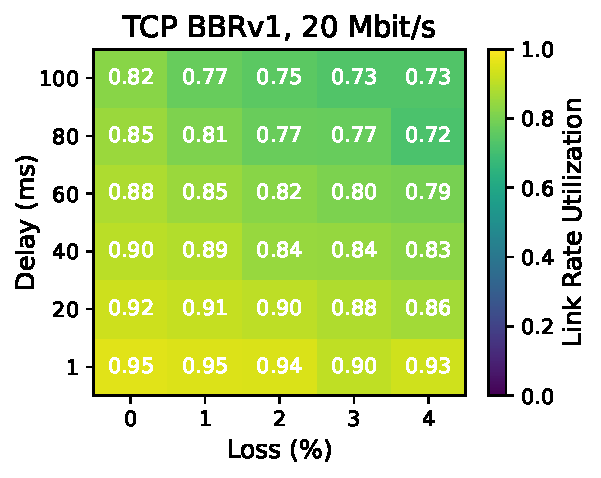
\includegraphics[width=\linewidth,trim={0 0 2cm 0},clip]{splitting-paper/figures/heatmaps/heatmap_tcp_bbr1_20mbps.pdf}
        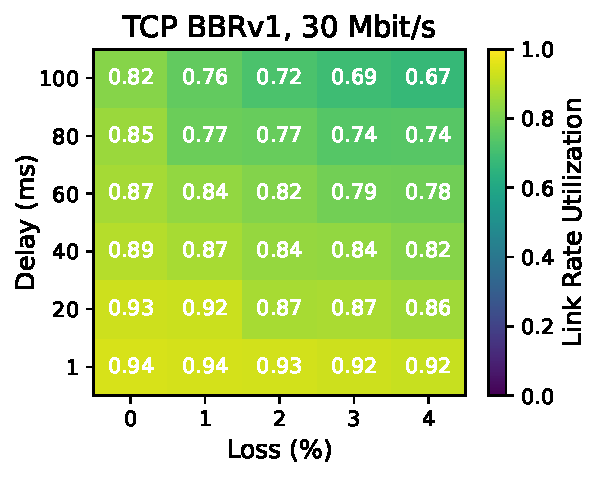
\includegraphics[width=\linewidth,trim={0 0 2cm 0},clip]{splitting-paper/figures/heatmaps/heatmap_tcp_bbr1_30mbps.pdf}
        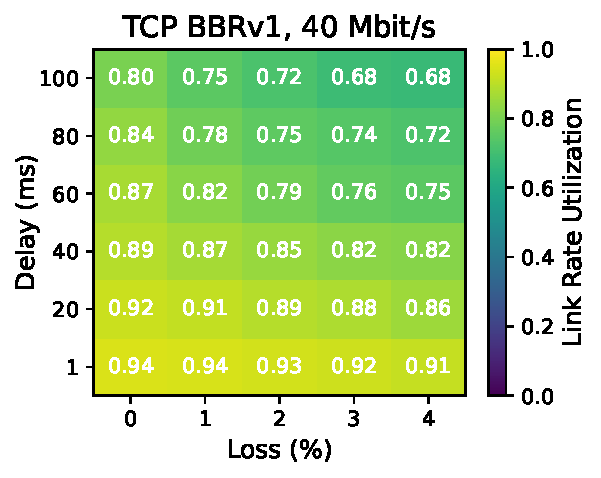
\includegraphics[width=\linewidth,trim={0 0 2cm 0},clip]{splitting-paper/figures/heatmaps/heatmap_tcp_bbr1_40mbps.pdf}
        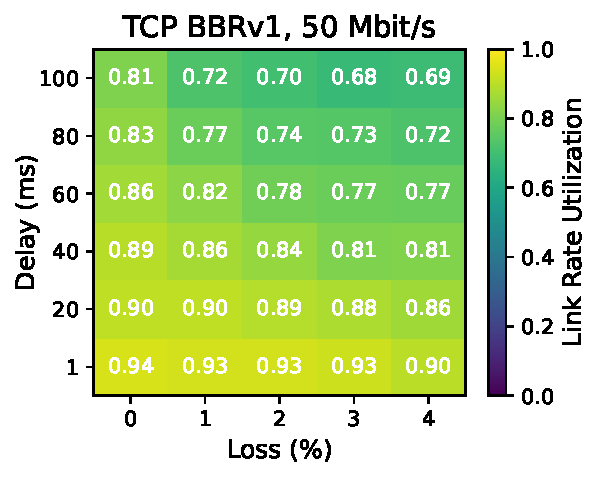
\includegraphics[width=\linewidth,trim={0 0 2cm 0},clip]{splitting-paper/figures/heatmaps/heatmap_tcp_bbr1_50mbps.pdf}
        \caption{Linux TCP.}
    \end{subfigure}
    \begin{subfigure}[b]{0.22\linewidth}
        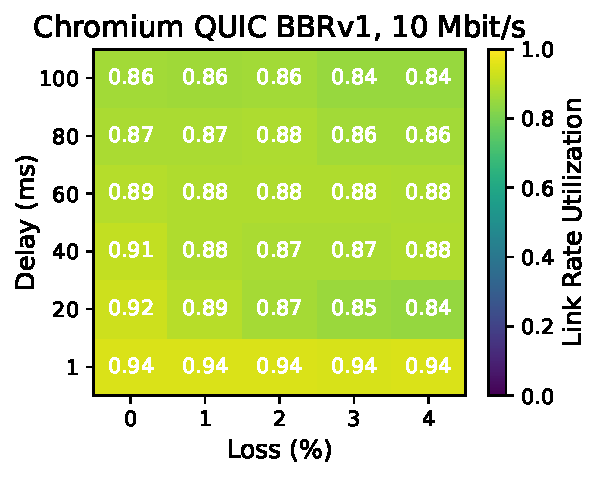
\includegraphics[width=\linewidth,trim={0 0 2cm 0},clip]{splitting-paper/figures/heatmaps/heatmap_quic_bbr1_10mbps.pdf}
        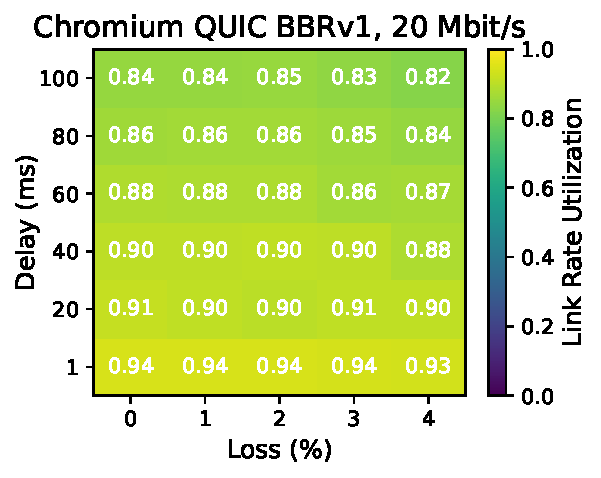
\includegraphics[width=\linewidth,trim={0 0 2cm 0},clip]{splitting-paper/figures/heatmaps/heatmap_quic_bbr1_20mbps.pdf}
        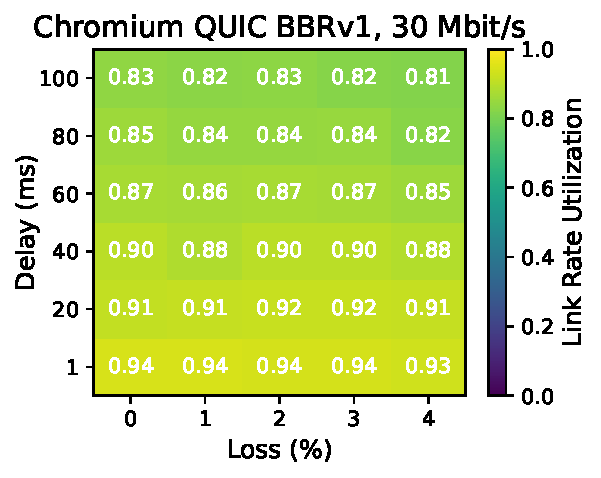
\includegraphics[width=\linewidth,trim={0 0 2cm 0},clip]{splitting-paper/figures/heatmaps/heatmap_quic_bbr1_30mbps.pdf}
        \includegraphics[width=\linewidth,trim={0 0 2cm 0},clip]{splitting-paper/figures/heatmaps/heatmap_quic_bbr1_40mbps.pdf}
        \includegraphics[width=\linewidth,trim={0 0 2cm 0},clip]{splitting-paper/figures/heatmaps/heatmap_quic_bbr1_50mbps.pdf}
        \caption{Google \texttt{quiche}.}
    \end{subfigure}
    \begin{subfigure}[b]{0.22\linewidth}
        \includegraphics[width=\linewidth,trim={0 0 2cm 0},clip]{splitting-paper/figures/heatmaps/heatmap_quiche_bbr1_10mbps.pdf}
        \includegraphics[width=\linewidth,trim={0 0 2cm 0},clip]{splitting-paper/figures/heatmaps/heatmap_quiche_bbr1_20mbps.pdf}
        \includegraphics[width=\linewidth,trim={0 0 2cm 0},clip]{splitting-paper/figures/heatmaps/heatmap_quiche_bbr1_30mbps.pdf}
        \includegraphics[width=\linewidth,trim={0 0 2cm 0},clip]{splitting-paper/figures/heatmaps/heatmap_quiche_bbr1_40mbps.pdf}
        \includegraphics[width=\linewidth,trim={0 0 2cm 0},clip]{splitting-paper/figures/heatmaps/heatmap_quiche_bbr1_50mbps.pdf}
        \caption{Cloudflare \texttt{quiche}.}
    \end{subfigure}
    \begin{subfigure}[b]{0.22\linewidth}
        \includegraphics[width=\linewidth,trim={0 0 2cm 0},clip]{splitting-paper/figures/heatmaps/heatmap_picoquic_bbr1_10mbps.pdf}
        \includegraphics[width=\linewidth,trim={0 0 2cm 0},clip]{splitting-paper/figures/heatmaps/heatmap_picoquic_bbr1_20mbps.pdf}
        \includegraphics[width=\linewidth,trim={0 0 2cm 0},clip]{splitting-paper/figures/heatmaps/heatmap_picoquic_bbr1_30mbps.pdf}
        \includegraphics[width=\linewidth,trim={0 0 2cm 0},clip]{splitting-paper/figures/heatmaps/heatmap_picoquic_bbr1_40mbps.pdf}
        \includegraphics[width=\linewidth,trim={0 0 2cm 0},clip]{splitting-paper/figures/heatmaps/heatmap_picoquic_bbr1_50mbps.pdf}
        \caption{\texttt{picoquic}.}
    \end{subfigure}
    \begin{subfigure}[b]{0.89cm}
        \includegraphics[width=\linewidth,trim={8cm 0 0 0},clip]{splitting-paper/figures/heatmaps/heatmap_tcp_bbr1_50mbps.pdf}
        \includegraphics[width=\linewidth,trim={8cm 0 0 0},clip]{splitting-paper/figures/heatmaps/heatmap_tcp_bbr1_50mbps.pdf}
        \includegraphics[width=\linewidth,trim={8cm 0 0 0},clip]{splitting-paper/figures/heatmaps/heatmap_tcp_bbr1_50mbps.pdf}
        \includegraphics[width=\linewidth,trim={8cm 0 0 0},clip]{splitting-paper/figures/heatmaps/heatmap_tcp_bbr1_50mbps.pdf}
        \includegraphics[width=\linewidth,trim={8cm 0 0 0},clip]{splitting-paper/figures/heatmaps/heatmap_tcp_bbr1_50mbps.pdf}
        \vspace*{0.2cm}
    \end{subfigure}
    \caption{BBRv2.}
\end{figure*}

\begin{figure*}[ht]
    \centering
    \begin{subfigure}[b]{0.22\linewidth}
        \includegraphics[width=\linewidth,trim={0 0 2cm 0},clip]{splitting-paper/figures/heatmaps/heatmap_tcp_cubic_10mbps.pdf}
        \includegraphics[width=\linewidth,trim={0 0 2cm 0},clip]{splitting-paper/figures/heatmaps/heatmap_tcp_cubic_20mbps.pdf}
        \includegraphics[width=\linewidth,trim={0 0 2cm 0},clip]{splitting-paper/figures/heatmaps/heatmap_tcp_cubic_30mbps.pdf}
        \includegraphics[width=\linewidth,trim={0 0 2cm 0},clip]{splitting-paper/figures/heatmaps/heatmap_tcp_cubic_40mbps.pdf}
        \includegraphics[width=\linewidth,trim={0 0 2cm 0},clip]{splitting-paper/figures/heatmaps/heatmap_tcp_cubic_50mbps.pdf}
        \caption{Linux TCP.}
    \end{subfigure}
    \begin{subfigure}[b]{0.22\linewidth}
        \includegraphics[width=\linewidth,trim={0 0 2cm 0},clip]{splitting-paper/figures/heatmaps/heatmap_quic_cubic_10mbps.pdf}
        \includegraphics[width=\linewidth,trim={0 0 2cm 0},clip]{splitting-paper/figures/heatmaps/heatmap_quic_cubic_20mbps.pdf}
        \includegraphics[width=\linewidth,trim={0 0 2cm 0},clip]{splitting-paper/figures/heatmaps/heatmap_quic_cubic_30mbps.pdf}
        \includegraphics[width=\linewidth,trim={0 0 2cm 0},clip]{splitting-paper/figures/heatmaps/heatmap_quic_cubic_40mbps.pdf}
        \includegraphics[width=\linewidth,trim={0 0 2cm 0},clip]{splitting-paper/figures/heatmaps/heatmap_quic_cubic_50mbps.pdf}
        \caption{Google \texttt{quiche}.}
    \end{subfigure}
    \begin{subfigure}[b]{0.22\linewidth}
        \includegraphics[width=\linewidth,trim={0 0 2cm 0},clip]{splitting-paper/figures/heatmaps/heatmap_quiche_cubic_10mbps.pdf}
        \includegraphics[width=\linewidth,trim={0 0 2cm 0},clip]{splitting-paper/figures/heatmaps/heatmap_quiche_cubic_20mbps.pdf}
        \includegraphics[width=\linewidth,trim={0 0 2cm 0},clip]{splitting-paper/figures/heatmaps/heatmap_quiche_cubic_30mbps.pdf}
        \includegraphics[width=\linewidth,trim={0 0 2cm 0},clip]{splitting-paper/figures/heatmaps/heatmap_quiche_cubic_40mbps.pdf}
        \includegraphics[width=\linewidth,trim={0 0 2cm 0},clip]{splitting-paper/figures/heatmaps/heatmap_quiche_cubic_50mbps.pdf}
        \caption{Cloudflare \texttt{quiche}.}
    \end{subfigure}
    \begin{subfigure}[b]{0.22\linewidth}
        \includegraphics[width=\linewidth,trim={0 0 2cm 0},clip]{splitting-paper/figures/heatmaps/heatmap_picoquic_cubic_10mbps.pdf}
        \includegraphics[width=\linewidth,trim={0 0 2cm 0},clip]{splitting-paper/figures/heatmaps/heatmap_picoquic_cubic_20mbps.pdf}
        \includegraphics[width=\linewidth,trim={0 0 2cm 0},clip]{splitting-paper/figures/heatmaps/heatmap_picoquic_cubic_30mbps.pdf}
        \includegraphics[width=\linewidth,trim={0 0 2cm 0},clip]{splitting-paper/figures/heatmaps/heatmap_picoquic_cubic_40mbps.pdf}
        \includegraphics[width=\linewidth,trim={0 0 2cm 0},clip]{splitting-paper/figures/heatmaps/heatmap_picoquic_cubic_50mbps.pdf}
        \caption{\texttt{picoquic}.}
    \end{subfigure}
    \begin{subfigure}[b]{0.89cm}
        \includegraphics[width=\linewidth,trim={8cm 0 0 0},clip]{splitting-paper/figures/heatmaps/heatmap_tcp_cubic_50mbps.pdf}
        \includegraphics[width=\linewidth,trim={8cm 0 0 0},clip]{splitting-paper/figures/heatmaps/heatmap_tcp_cubic_50mbps.pdf}
        \includegraphics[width=\linewidth,trim={8cm 0 0 0},clip]{splitting-paper/figures/heatmaps/heatmap_tcp_cubic_50mbps.pdf}
        \includegraphics[width=\linewidth,trim={8cm 0 0 0},clip]{splitting-paper/figures/heatmaps/heatmap_tcp_cubic_50mbps.pdf}
        \includegraphics[width=\linewidth,trim={8cm 0 0 0},clip]{splitting-paper/figures/heatmaps/heatmap_tcp_cubic_50mbps.pdf}
        \vspace*{0.2cm}
    \end{subfigure}
    \caption{CUBIC.}
\end{figure*}

\begin{figure*}[ht]
    \centering
    \begin{subfigure}[b]{0.22\linewidth}
        \includegraphics[width=\linewidth,trim={0 0 2cm 0},clip]{splitting-paper/figures/heatmaps/heatmap_tcp_reno_10mbps.pdf}
        \includegraphics[width=\linewidth,trim={0 0 2cm 0},clip]{splitting-paper/figures/heatmaps/heatmap_tcp_reno_20mbps.pdf}
        \includegraphics[width=\linewidth,trim={0 0 2cm 0},clip]{splitting-paper/figures/heatmaps/heatmap_tcp_reno_30mbps.pdf}
        \includegraphics[width=\linewidth,trim={0 0 2cm 0},clip]{splitting-paper/figures/heatmaps/heatmap_tcp_reno_40mbps.pdf}
        \includegraphics[width=\linewidth,trim={0 0 2cm 0},clip]{splitting-paper/figures/heatmaps/heatmap_tcp_reno_50mbps.pdf}
        \caption{Linux TCP.}
    \end{subfigure}
    \begin{subfigure}[b]{0.22\linewidth}
        \includegraphics[width=\linewidth,trim={0 0 2cm 0},clip]{splitting-paper/figures/heatmaps/heatmap_quic_reno_10mbps.pdf}
        \includegraphics[width=\linewidth,trim={0 0 2cm 0},clip]{splitting-paper/figures/heatmaps/heatmap_quic_reno_20mbps.pdf}
        \includegraphics[width=\linewidth,trim={0 0 2cm 0},clip]{splitting-paper/figures/heatmaps/heatmap_quic_reno_30mbps.pdf}
        \includegraphics[width=\linewidth,trim={0 0 2cm 0},clip]{splitting-paper/figures/heatmaps/heatmap_quic_reno_40mbps.pdf}
        \includegraphics[width=\linewidth,trim={0 0 2cm 0},clip]{splitting-paper/figures/heatmaps/heatmap_quic_reno_50mbps.pdf}
        \caption{Google \texttt{quiche}.}
    \end{subfigure}
    \begin{subfigure}[b]{0.22\linewidth}
        \includegraphics[width=\linewidth,trim={0 0 2cm 0},clip]{splitting-paper/figures/heatmaps/heatmap_quiche_reno_10mbps.pdf}
        \includegraphics[width=\linewidth,trim={0 0 2cm 0},clip]{splitting-paper/figures/heatmaps/heatmap_quiche_reno_20mbps.pdf}
        \includegraphics[width=\linewidth,trim={0 0 2cm 0},clip]{splitting-paper/figures/heatmaps/heatmap_quiche_reno_30mbps.pdf}
        \includegraphics[width=\linewidth,trim={0 0 2cm 0},clip]{splitting-paper/figures/heatmaps/heatmap_quiche_reno_40mbps.pdf}
        \includegraphics[width=\linewidth,trim={0 0 2cm 0},clip]{splitting-paper/figures/heatmaps/heatmap_quiche_reno_50mbps.pdf}
        \caption{Cloudflare \texttt{quiche}.}
    \end{subfigure}
    \begin{subfigure}[b]{0.89cm}
        \includegraphics[width=\linewidth,trim={8cm 0 0 0},clip]{splitting-paper/figures/heatmaps/heatmap_tcp_reno_50mbps.pdf}
        \includegraphics[width=\linewidth,trim={8cm 0 0 0},clip]{splitting-paper/figures/heatmaps/heatmap_tcp_reno_50mbps.pdf}
        \includegraphics[width=\linewidth,trim={8cm 0 0 0},clip]{splitting-paper/figures/heatmaps/heatmap_tcp_reno_50mbps.pdf}
        \includegraphics[width=\linewidth,trim={8cm 0 0 0},clip]{splitting-paper/figures/heatmaps/heatmap_tcp_reno_50mbps.pdf}
        \includegraphics[width=\linewidth,trim={8cm 0 0 0},clip]{splitting-paper/figures/heatmaps/heatmap_tcp_reno_50mbps.pdf}
        \vspace*{0.2cm}
    \end{subfigure}
    \caption{Reno.}
\end{figure*}
